\documentclass[11pt, a4paper]{article}
\usepackage[a4paper, top=2.0cm, bottom=2.0cm, left=2.2cm, right=2.2cm]{geometry}
\usepackage{fontspec}
\usepackage[indonesian]{babel}
\babelfont{rm}{Noto Sans}

\usepackage{xcolor}
\usepackage{enumitem}
\usepackage{hyperref}
\usepackage{array}
\usepackage{tabularx}
\usepackage{booktabs}
\usepackage{tcolorbox}
\tcbuselibrary{skins}
\usepackage{tikz}
\usetikzlibrary{shapes.geometric, positioning, calc}
\usepackage{fancyhdr}
\usepackage{titlesec}
\usepackage{graphicx}

%--- WARNA (Biru UNIDA Gontor) ---
\definecolor{unidanavy}{HTML}{0B2A4A}
\definecolor{unidablue}{HTML}{1E6091}
\definecolor{unidagold}{HTML}{D4AF37}
\definecolor{unidabg}{HTML}{F1F5F9}
\definecolor{unidatext}{HTML}{0F172A}
\definecolor{unidagray}{HTML}{64748B}
\definecolor{unidaborder}{HTML}{CBD5E1}

\hypersetup{
  colorlinks=true, linkcolor=unidablue, urlcolor=unidablue,
  pdftitle={Proposal SOUQNA Web}, pdfauthor={Farrel Ghozy Affifudin}
}

\setlength{\parskip}{0.25em}
\setlength{\parindent}{0pt}
\setlist[itemize]{label=\textcolor{unidablue}{\textbullet}, leftmargin=1.4em, itemsep=0.04em, topsep=0.08em}
\setlist[enumerate]{leftmargin=1.4em, itemsep=0.04em, topsep=0.08em}

%--- HEADING ---
\titleformat{\section}
  {\normalfont\large\bfseries\color{unidanavy}}
  {\llap{\color{unidagold}\rule[-2pt]{3.5pt}{1.1em}\hspace{0.5em}}\thesection.}{0.5em}{}
  [{\color{unidaborder}\titlerule[0.7pt]}]
\titlespacing*{\section}{0pt}{0.8em}{0.25em}

\titleformat{\subsection}
  {\normalfont\normalsize\bfseries\color{unidablue}}
  {\thesubsection}{0.5em}{}
\titlespacing*{\subsection}{0pt}{0.6em}{0.2em}

%--- HEADER / FOOTER ---
\setlength{\headheight}{24pt}
\pagestyle{fancy}
\fancyhf{}
\fancyhead[L]{\textcolor{unidagray}{\small\textsf{SOUQNA --- Proposal Aplikasi Web React}}}
\fancyhead[R]{\textcolor{unidagold}{\small\textbf{\textsf{UNIDA Gontor Siman}}}}
\fancyfoot[L]{\textcolor{unidagray}{\footnotesize\textsf{Farrel Ghozy Affifudin --- 452024611053}}}
\fancyfoot[R]{\textcolor{unidanavy}{\small\textbf{\thepage}}}
\renewcommand{\headrulewidth}{0.5pt}
\renewcommand{\footrulewidth}{0.5pt}
\renewcommand{\headrule}{\hbox to\headwidth{\color{unidaborder}\leaders\hrule height \headrulewidth\hfill}}
\renewcommand{\footrule}{\hbox to\headwidth{\color{unidaborder}\leaders\hrule height \footrulewidth\hfill}}

\begin{document}

\null \vspace{\stretch{1}}

%======================================================================================
% COVER
%======================================================================================
\begin{tcolorbox}[
  enhanced,
  colback=unidabg, colframe=unidanavy, boxrule=1.5pt, arc=6pt,
  left=12pt, right=12pt, top=12pt, bottom=12pt,
  borderline west={5pt}{0pt}{unidagold}
]
  \begin{center}
    \IfFileExists{logo-horizontal.png}{%
      
\includegraphics[height=1.2cm]{logo-horizontal.png}\\[0.3cm]
    }{%
      {\Huge\bfseries\color{unidanavy} SOUQNA}\\[0.1cm]
    }
    {\Large\textbf{\color{unidanavy} PROPOSAL RANCANGAN APLIKASI BERBASIS WEB}}\\[0.1cm]
    {\LARGE\textbf{\color{unidablue} SOUQNA (\textit{Pasar Kita})}}\\[0.1cm]
    {\small\color{unidagray} Platform Marketplace Internal Kampus Berbasis React + Supabase}\\[0.25cm]
    \rule{0.88\textwidth}{0.6pt}\\[0.15cm]
    {\small\textbf{\color{unidagray} Mata Kuliah: Pemrograman Web}}
  \end{center}

  \vspace{0.15cm}
  \begin{tabularx}{\textwidth}{@{} >{\bfseries}p{3.8cm} p{0.2cm} >{\raggedright\arraybackslash}X @{}}
    Nama               & : & \textbf{Farrel Ghozy Affifudin} --- NIM: 452024611053 \\
    Program Studi      & : & Teknik Informatika \\
    Fakultas / Kampus  & : & Sains dan Teknologi, UNIDA Gontor, Kampus Siman \\
    Platform Target    & : & Web (React + database Supabase) \\
    Metode Pembayaran  & : & COD (bayar di tempat saat terima barang) \\
  \end{tabularx}
\end{tcolorbox}

\vspace{\stretch{1}} \null

\clearpage

%======================================================================================
% 1. JUDUL
%======================================================================================
\section{Judul}

\textbf{SOUQNA (\textit{Pasar Kita}): Rancangan Aplikasi Marketplace Internal Kampus UNIDA Gontor Siman Berbasis Web (React + Supabase).}

Ruang lingkup proposal ini adalah bagian \textbf{web (frontend React + database Supabase)}.
Proyek SOUQNA secara keseluruhan dikerjakan untuk dua mata kuliah (mobile dan web);
dokumen ini hanya membahas sisi web agar sesuai penugasan Mata Kuliah Pemrograman Web.

%======================================================================================
% 2. LATAR BELAKANG MASALAH
%======================================================================================
\section{Latar Belakang Masalah}

UNIDA Gontor Kampus Siman adalah kampus berbasis asrama (boarding) dengan aturan
perizinan keluar kampus yang ketat. Mahasiswa diharapkan memenuhi kebutuhan harian
di dalam kampus --- mulai dari makanan, perlengkapan ibadah, ATK, hingga jasa cetak ---
tanpa harus belanja ke luar.

Masalahnya, informasi barang yang ada di dalam kampus tidak terpusat. Jual-beli antar
unit usaha kampus (kantin, percetakan, koperasi, dan stan lainnya) masih mengandalkan
broadcast WhatsApp yang tidak terstruktur: tidak ada katalog terpusat, stok tidak
terlihat, harga simpang siur, dan pesanan tidak tercatat.

\textbf{SOUQNA versi web} menjawab masalah tersebut: satu katalog web untuk seluruh
unit usaha internal kampus. Mahasiswa memesan dari asrama lewat browser, melihat stok
dan harga dengan jelas, lalu membayar di tempat saat barang diterima atau diambil
(COD). COD dipilih karena pada versi awal ini belum ada pembayaran digital --- intinya pembeli membayar setelah barang sampai atau diambil.

%======================================================================================
% 3. TUJUAN
%======================================================================================
\section{Tujuan}

\begin{enumerate}
  \item Menyediakan katalog web terpusat untuk unit usaha kampus agar stok dan harga terlihat jelas.
  \item Memudahkan mahasiswa memesan kebutuhan dari dalam kampus tanpa harus belanja ke luar.
  \item Membantu unit usaha kampus (kantin, percetakan, koperasi) mengelola produk dan pesanan secara digital lewat dasbor web.
  \item Menyediakan alur pemesanan web yang jelas: pesan, konfirmasi, serah terima, sampai bayar di tempat.
  \item Menerapkan arsitektur web modern yang rapi dan mudah dikembangkan ke depannya.
\end{enumerate}

%======================================================================================
% 4. RANCANGAN
%======================================================================================
\section{Rancangan}

\subsection{Gambaran Umum dan Peran Pengguna}

Aplikasi web SOUQNA memiliki tiga peran utama:

\begin{itemize}
  \item \textbf{Pembeli (mahasiswa):} melihat beranda dan katalog, mencari dan memfilter produk, melihat detail produk dan toko, mengelola keranjang, checkout dengan bayar di tempat, melacak pesanan, menyimpan wishlist, chat dengan toko, dan memberi ulasan.
  \item \textbf{Penjual (unit usaha):} mengelola satu toko: melihat ringkasan usaha, menambah dan mengubah produk beserta stok dan harganya, memproses pesanan yang masuk, serta mengatur profil dan lokasi stan.
  \item \textbf{Admin kampus:} memantau pengguna, kategori, produk, pesanan, voucher, dan riwayat aktivitas lewat panel admin web.
\end{itemize}

Pengiriman hanya dua pilihan: \textbf{ambil sendiri di stan (gratis)} atau \textbf{diantar penjual ke asrama (tambah Rp 2.000)} --- tanpa kurir dari luar. Koordinasi pengambilan dan pengantaran lewat nomor kontak toko.

\subsection{Arsitektur Web dan Database}

Aplikasi dibangun sebagai aplikasi web modern dengan tiga lapisan utama:

\begin{itemize}
  \item \textbf{Tampilan web:} dibangun dengan React, yaitu pustaka JavaScript populer untuk membangun antarmuka web yang cepat dan responsif. Navigasinya dibagi menjadi area publik, area akun, area penjual, dan area admin, masing-masing dijaga sesuai peran pengguna yang sedang masuk.
  \item \textbf{Perantara data:} seluruh halaman mengambil data lewat satu pintu yang sama, sehingga tampilan tidak perlu tahu data berasal dari contoh sementara atau dari database sungguhan. Selama pengembangan, data masih memakai data contoh agar bisa didemokan tanpa server.
  \item \textbf{Database:} dirancang memakai Supabase, yaitu layanan database yang menyediakan penyimpanan data, layanan masuk akun, dan penyimpanan foto produk maupun toko dalam satu tempat.
  \item \textbf{Tampilan visual:} memakai warna identitas Biru UNIDA Gontor (navy, biru, dan aksen emas), harga dalam Rupiah dan waktu cadangan Jakarta, serta setiap halaman selalu punya kondisi memuat, kosong, gagal, dan berhasil agar pengguna tidak bingung.
\end{itemize}

\begin{center}
\begin{tikzpicture}[
  box/.style={draw=unidaborder, fill=white, rounded corners=4pt, minimum width=2.9cm, minimum height=1.0cm, align=center, font=\scriptsize},
  arrow/.style={->, thick, color=unidablue}
]
  \node[box, fill=unidabg] (ui) {Halaman Web};
  \node[box, right=0.7cm of ui] (api) {Perantara Data};
  \node[box, right=0.7cm of api] (sb) {Database\\Supabase};
  \draw[arrow] (ui) -- (api);
  \draw[arrow] (api) -- (sb);
  \draw[arrow, dashed] (sb) -- (api);
  \draw[arrow, dashed] (api) -- (ui);
\end{tikzpicture}\\[0.1cm]
{\scriptsize\textcolor{unidagray}{Gambar 1. Alur data: halaman web meminta data lewat perantara, lalu diteruskan ke database.}}
\end{center}

\subsection{Daftar Halaman dan Fitur Web}

\begin{itemize}
  \item \textbf{Area publik:} beranda, pencarian produk, daftar kategori, detail produk, dan detail toko. Bisa dibuka tanpa masuk akun.
  \item \textbf{Masuk akun:} halaman masuk, daftar akun baru, dan lupa kata sandi. Saat demo, masuk cukup memakai email tanpa kata sandi.
  \item \textbf{Area pembeli:} keranjang belanja, pembayaran di tempat, riwayat dan detail pesanan, wishlist, chat dengan toko, dan profil pengguna.
  \item \textbf{Area penjual:} dasbor usaha, profil toko, daftar dan formulir produk, serta daftar pesanan masuk.
  \item \textbf{Area admin:} dasbor ringkasan, kelola pengguna, kategori, produk, pesanan, voucher, dan riwayat aktivitas.
\end{itemize}

Setiap checkout dihitung per toko. Total bayar adalah jumlah harga barang ditambah ongkir, dikurangi potongan voucher bila ada. Status pesanan ditulis dalam Bahasa Indonesia (misalnya Menunggu, Diproses, Selesai) agar mudah dipahami.

\subsection{Data yang Disimpan}

Data yang dirancang meliputi data pengguna, toko, kategori, produk beserta varian harga dan stoknya, keranjang, wishlist, pesanan beserta rincian barangnya, voucher, ulasan, percakapan chat, dan riwayat aktivitas. Hubungannya sederhana: satu toko memiliki banyak produk, satu produk bisa punya beberapa varian, satu pesanan milik satu pembeli dan satu toko, dan setiap perubahan status pesanan tercatat sebagai riwayat.

\subsection{Tampilan Antarmuka Web}

Berikut tampilan asli aplikasi web SOUQNA dengan warna identitas Biru UNIDA Gontor.

\begin{center}
  \begin{minipage}[t]{0.48\textwidth}
    \centering
    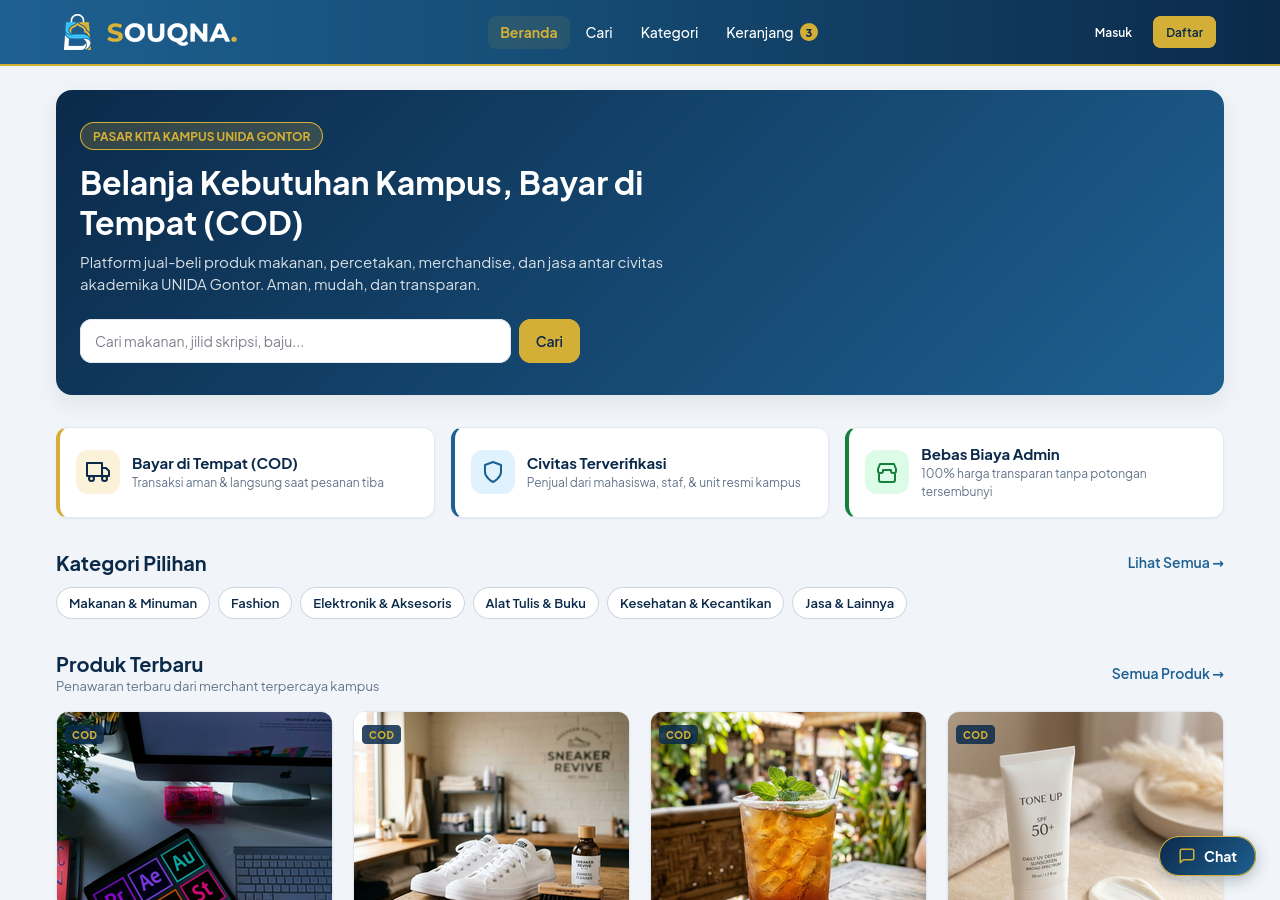
\includegraphics[width=\textwidth]{web-beranda.png}\\[0.1cm]
    {\footnotesize\textbf{(A) Beranda}}\\{\scriptsize\textcolor{unidagray}{Spanduk COD, kategori, dan produk terbaru}}
  \end{minipage}
  \hfill
  \begin{minipage}[t]{0.48\textwidth}
    \centering
    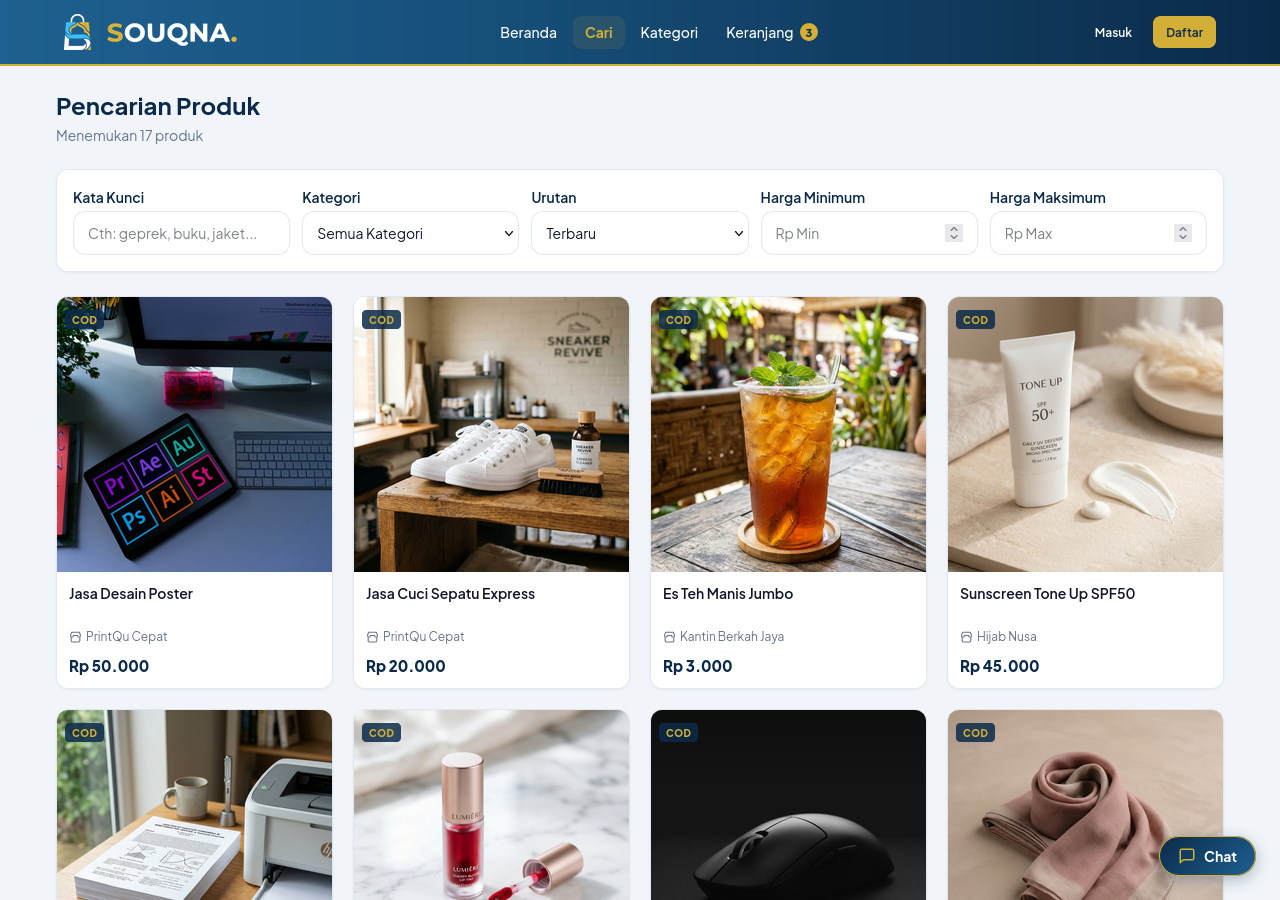
\includegraphics[width=\textwidth]{web-katalog.png}\\[0.1cm]
    {\footnotesize\textbf{(B) Pencarian}}\\{\scriptsize\textcolor{unidagray}{Cari produk dan saring berdasarkan kategori dan harga}}
  \end{minipage}

  \vspace{0.3cm}

  \begin{minipage}[t]{0.48\textwidth}
    \centering
    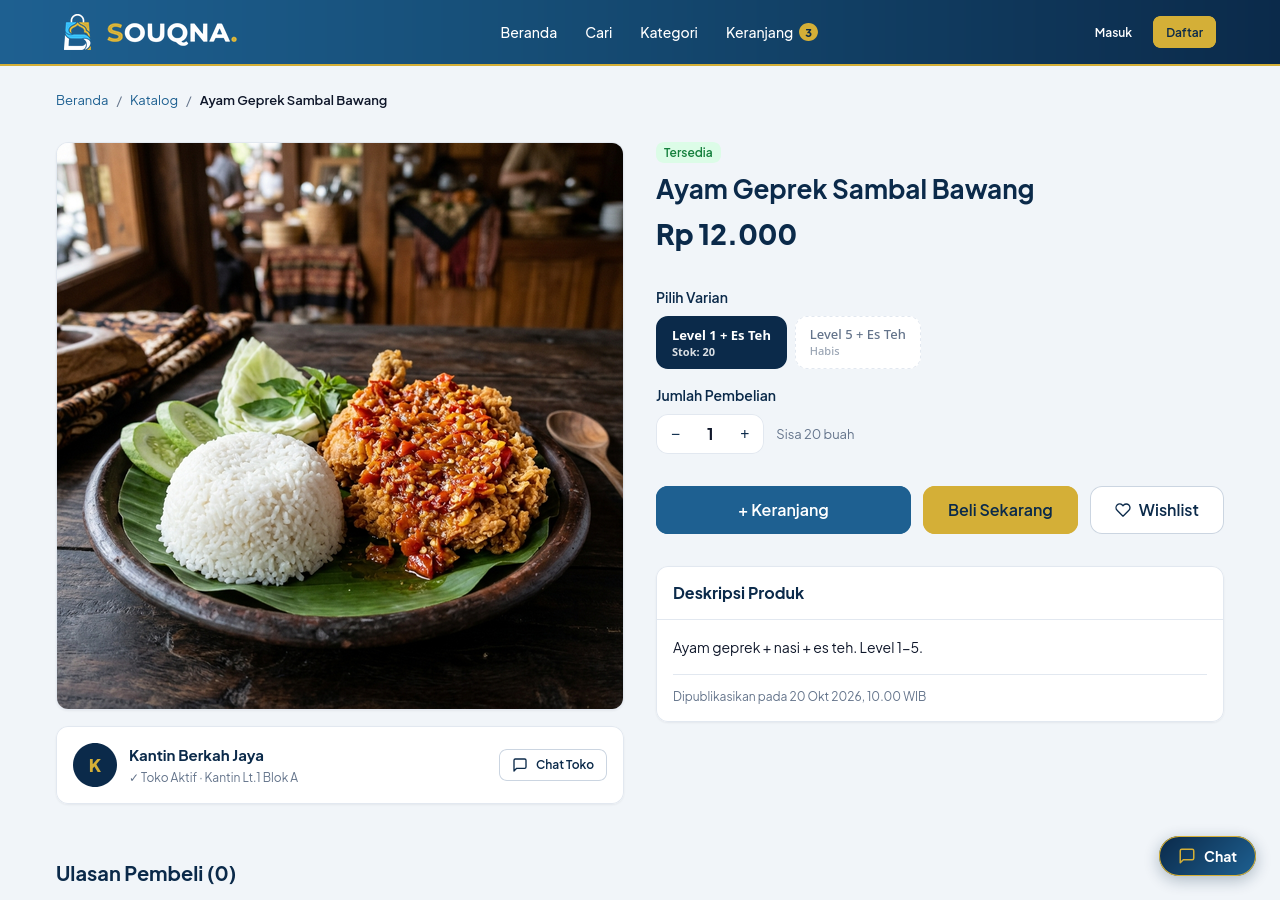
\includegraphics[width=\textwidth]{web-produk.png}\\[0.1cm]
    {\footnotesize\textbf{(C) Detail Produk}}\\{\scriptsize\textcolor{unidagray}{Foto, harga, stok, dan info toko}}
  \end{minipage}
  \hfill
  \begin{minipage}[t]{0.48\textwidth}
    \centering
    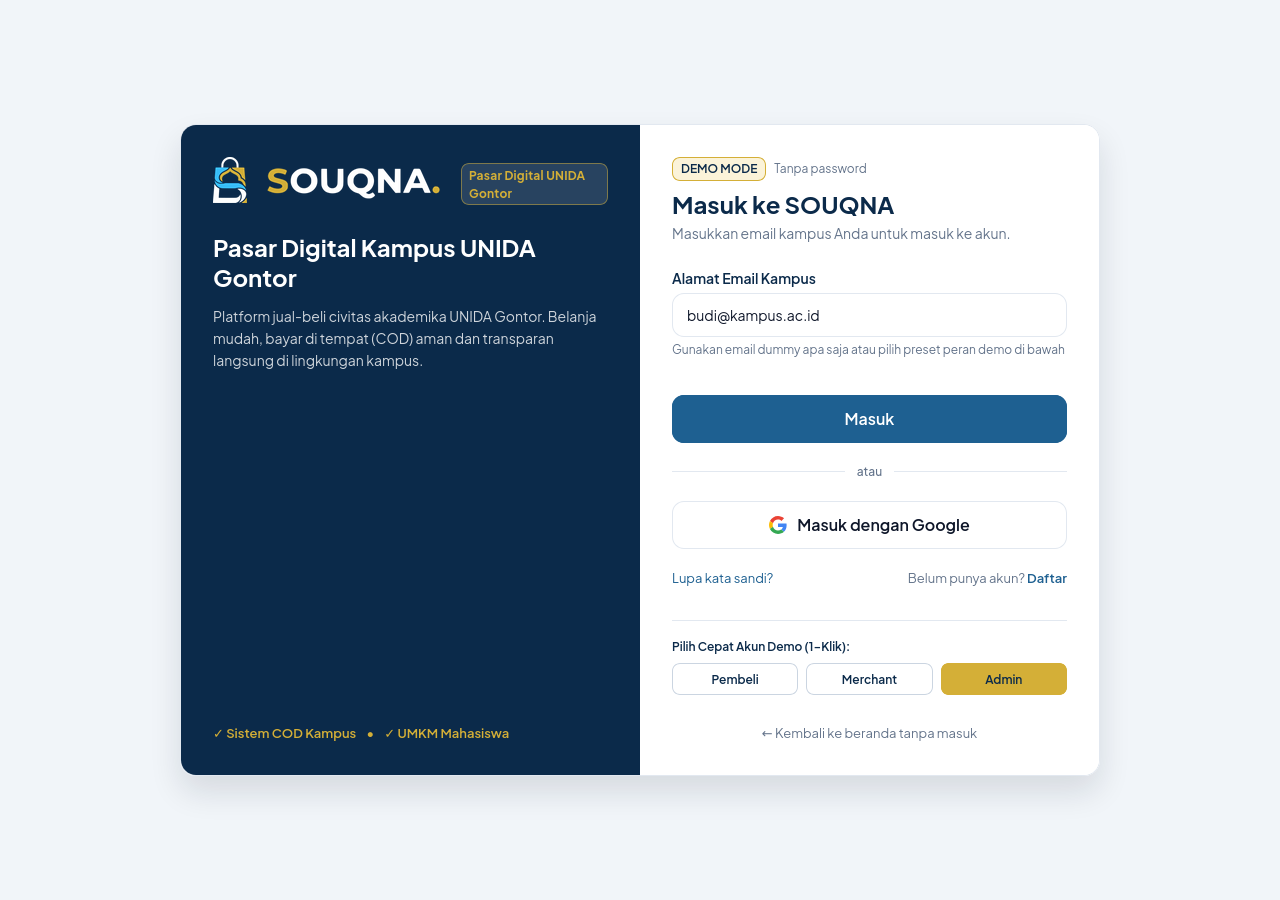
\includegraphics[width=\textwidth]{web-login.png}\\[0.1cm]
    {\footnotesize\textbf{(D) Masuk Akun}}\\{\scriptsize\textcolor{unidagray}{Masuk dengan email dan pilihan peran demo}}
  \end{minipage}

  \vspace{0.3cm}

  \begin{minipage}[t]{0.48\textwidth}
    \centering
    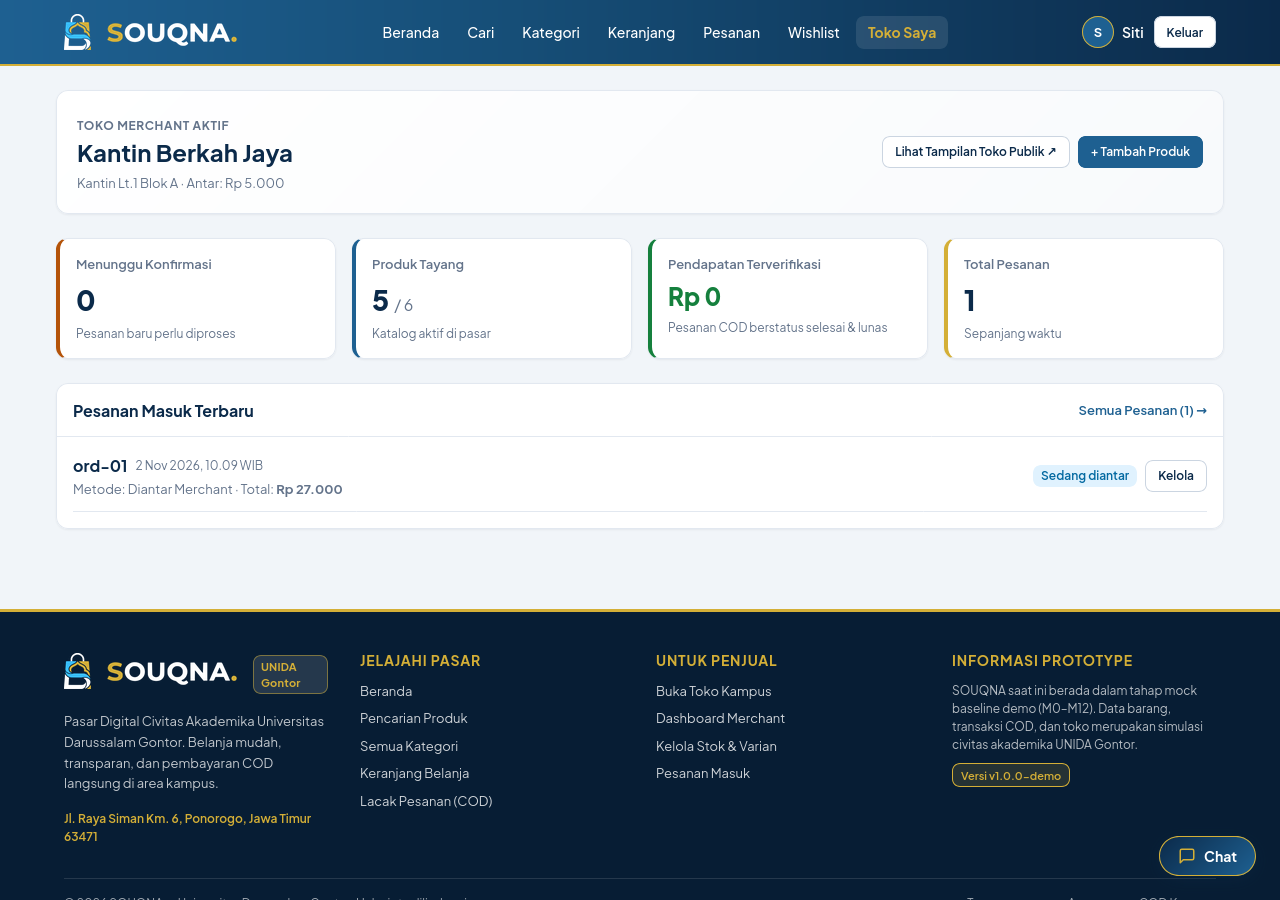
\includegraphics[width=\textwidth]{web-merchant.png}\\[0.1cm]
    {\footnotesize\textbf{(E) Dasbor Penjual}}\\{\scriptsize\textcolor{unidagray}{Kelola produk, stok, dan pesanan toko}}
  \end{minipage}
  \hfill
  \begin{minipage}[t]{0.48\textwidth}
    \centering
    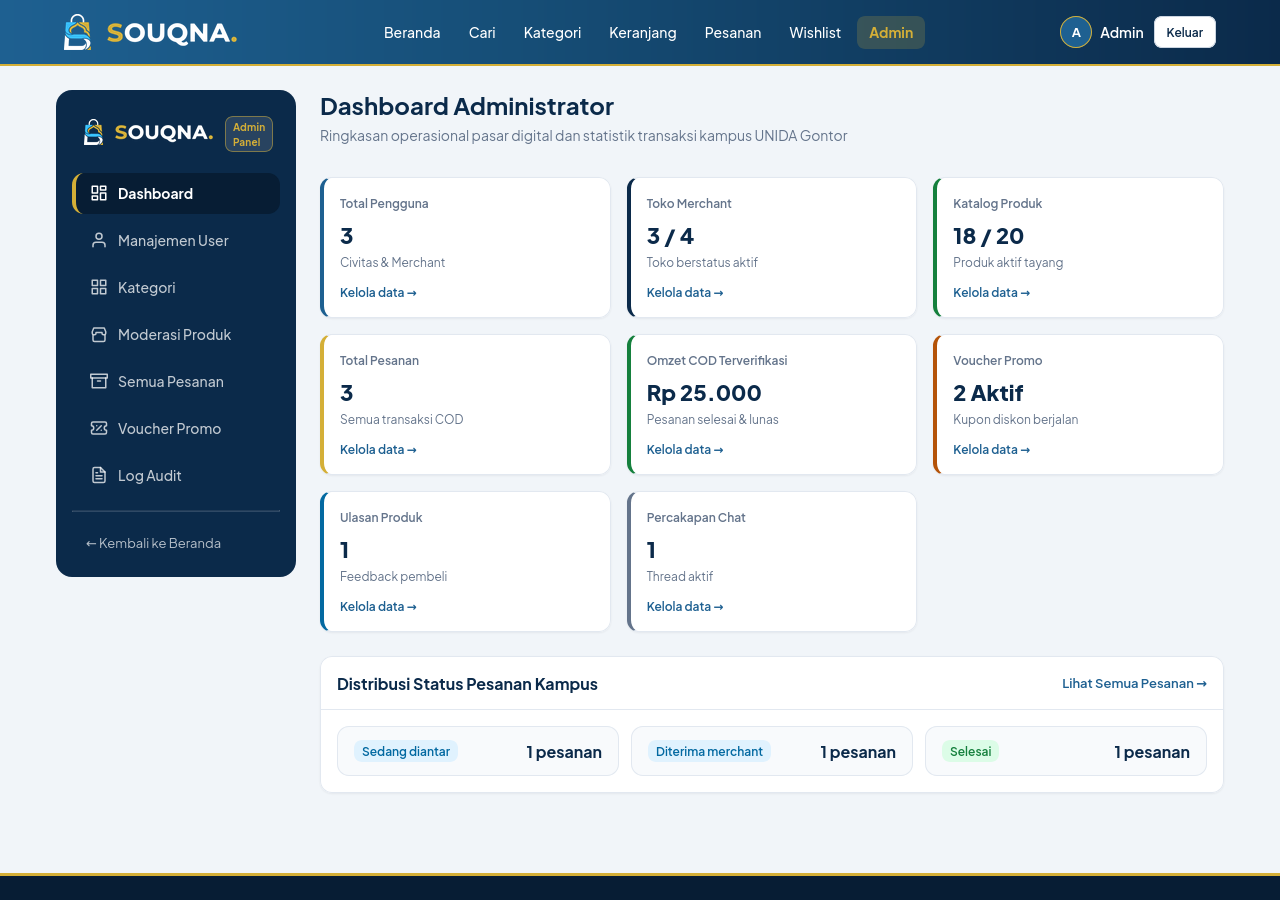
\includegraphics[width=\textwidth]{web-admin.png}\\[0.1cm]
    {\footnotesize\textbf{(F) Dasbor Admin}}\\{\scriptsize\textcolor{unidagray}{Ringkasan dan pengawasan seluruh aktivitas}}
  \end{minipage}
\end{center}

\subsection{Alur Pesanan dan Rencana Pengujian}

Alurnya sederhana: pembeli mengisi keranjang, lalu checkout dengan memilih ambil sendiri atau diantar, pesanan berstatus Menunggu, penjual mengonfirmasi dan memprosesnya, kemudian barang diserahterimakan dan dibayar di tempat hingga statusnya Selesai. Stok berkurang saat checkout dan dikembalikan bila pesanan dibatalkan, dan setiap pengguna hanya bisa melihat pesanan miliknya sendiri.

Uji coba dilakukan manual dengan data contoh yang didemokan ke dosen:

\vspace{0.1cm}
\noindent\small
\begin{tabularx}{\textwidth}{@{} c >{\raggedright\arraybackslash}p{3cm} >{\raggedright\arraybackslash}p{4.5cm} >{\raggedright\arraybackslash}X @{}}
\toprule
\textbf{ID} & \textbf{Skenario} & \textbf{Cara Uji} & \textbf{Hasil yang Diharapkan} \\
\midrule
TC-01 & Cari produk &
  Ketik ``geprek'' di pencarian web &
  Produk muncul dengan harga dan nama toko yang benar \\
\addlinespace
TC-02 & Beli sampai checkout &
  Masukkan 2 produk 1 toko ke keranjang, tekan Checkout &
  Muncul 1 pesanan dengan total = harga + ongkir $-$ voucher \\
\addlinespace
TC-03 & Lacak pesanan &
  Buka detail pesanan, tekan ``Saya Sudah Menerima Barang'' &
  Status berubah menjadi \textit{Selesai} \\
\addlinespace
TC-04 & Kelola unit usaha &
  Buka dasbor toko, ubah stok, simpan &
  Stok baru langsung terlihat di katalog pembeli \\
\bottomrule
\end{tabularx}

\vspace{0.4cm}
\normalsize

%======================================================================================
% 5. LAMPIRAN VIDEO DAN DOKUMENTASI
%======================================================================================
\section{Lampiran Video dan Dokumentasi Proyek}

Tautan folder Google Drive berisi dokumentasi lengkap proyek SOUQNA, meliputi video demo aplikasi web (alur TC-01 sampai TC-04 di atas) beserta dokumen proposal:

\begin{center}
\begin{tcolorbox}[colback=unidabg, colframe=unidaborder, boxrule=0.7pt, arc=4pt, left=10pt, right=10pt, top=8pt, bottom=8pt, width=0.95\textwidth]
\centering
\small\textcolor{unidagray}{Tautan video dan dokumentasi proyek:} \\[0.15cm]
{\footnotesize\url{https://drive.google.com/drive/folders/1zUCGN-jjEynvirZySUD416qlo5GEpM2a?usp=sharing}}
\end{tcolorbox}
\end{center}

\end{document}
